\subsubsection{Thermal resistance}
\label{sec:eval:pumpspot:rth}

In order to determine the thermal resistance $\Rth$
we have to look at
the longest emitted wavelength $\lambda$
at different heat sink temperature
versus dissipated power $D$,
(\ref{eq:dissip}).
According to the method
described in section~\ref{sec:rth:lambda}
we can find a linear relation
between $\lambda$ and $D$,
from which we can deduce
the thermal resistance $\Rth$.
We do this
for the different spot sizes,
and can thus conclude
on the scaling behavior.

The spot sizes
$\{180,300,400\}\,\mu\mathrm{m}$
were each measured for the temperatures
$\{15,30,45\}\,^\circ\mathrm{C}$,
using spherical lenses
for both $\mathrm{L}_\mathrm{p1}$ and $\mathrm{L}_\mathrm{p2}$,
as described in section~\ref{sec:exp:setup}.
Figure~\ref{img:Rth_lambda_spot_scaling}
plots the resulted longest wavelengths
against dissipated power.
The average maintained heat sink temperature,
plus-minus its standard deviation,
is stated in each of the subplots.
The straight lines correspond
to the linear fit (\ref{eq:rth_fit}).
The inset text in black
takes note of this fit,
displaying the fit parameters in values.
The stated thermal resistance results from
the ratio of the two fit parameters (\ref{eq:rth_long})
\begin{equation*}
\Rth = \pd{T}{D} = \pd{\lambda}{D}/\pd{\lambda}{T}.
%\label{eq:rth_long}
\end{equation*}

In order to obtain the fit
we consider only the data points
corresponding to
the linear light-light conversion regime --
the same as for estimating
the conversion efficiency
in section~\ref{sec:eval:pumpspot:pwr},
Fig.~\ref{img:LL_spot_scaling}.
This means
we exclude both,
threshold
and roll over segments.

Figure~\ref{img:Rth_spotsizescaling}
shows the scaling of $\Rth$
with respect to spot size.
The plot to the left
displays the behavior
noted in \cite{Giet2008}
and highlighted
in section~\ref{sec:rth:scaling}:
the thermal resistance
decreases less efficiently
than by area.
The reduction in $\Rth$
is closer to $w^{-1}$
than $w^{-2}$,
as illustrated
by the slope
given in the log-log plot.

A VECSEL device is thin
compared to the pumped area.
The expected heat flow
is one dimensional,
independent on lateral cooling.
The observed scaling behavior
shows this approximation
is not tenable.
In an attempt to understand
this behavior
when we look at
the expected temperature profile
from Fig.~\ref{img:Comsol_Tvsr}.
The temperature peaks
at the center
in the case of the depicted Gauss
and super-Gaussians and,
consequentially,
lateral heat transfer occurs,
beside the one-dimensional extraction
\cite{Chernikov2011}.

The measurements conducted
with the achromatic lens
could not be used
to extract the thermal resistance
with the method described
in section~\ref{sec:rth:lambda}.
Fit (\ref{eq:rth_fit}) relies
on a linear relation
between $\lambda$ and $D$
\cite{Heinen2012}.
As will be discussed
in section~\ref{sec:eval:trollover},
Fig.~\ref{img:lambda_sample},
this linearity was not given.

The fit in turquoise
corresponds to (\ref{eq:Rth_empirical}).
With only three data points available
to fit three parameters
we cannot judge
how good the found parameters
actually are.
But given the original meaning
of $a_3$ --
an outer radius  of a VCSEL --
we recognize the found values
not to make too much sense.
The found fit is valid
only for spot sizes smaller
than $2w=550\,\mu\mathrm{m}$.
This,
together with the large uncertainties
attached to the estimates of the thermal resistance,
show there needs more work to be done
in order to get a useful statement
out of the analysis of $\Rth$.


\begin{figure}
\centering
\subfigure{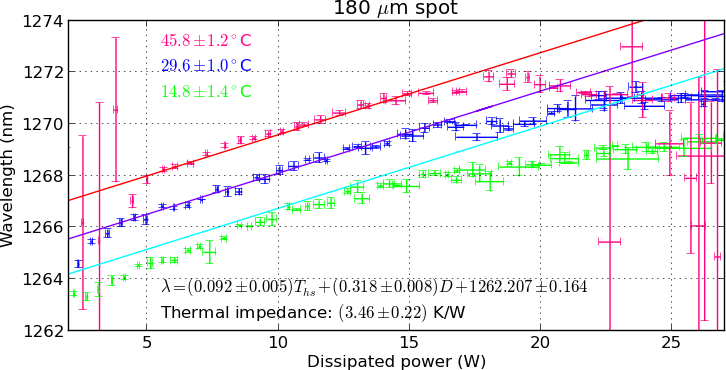
\includegraphics[width=14.5cm]{img/Rth_lambda_spot180um.png}}
\subfigure{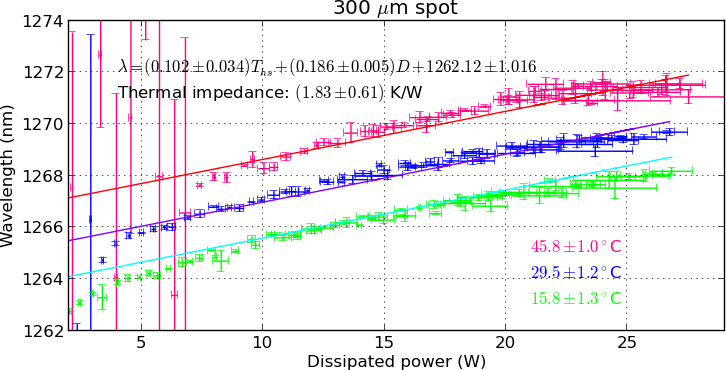
\includegraphics[width=14.5cm]{img/Rth_lambda_spot300um.png}}
\subfigure{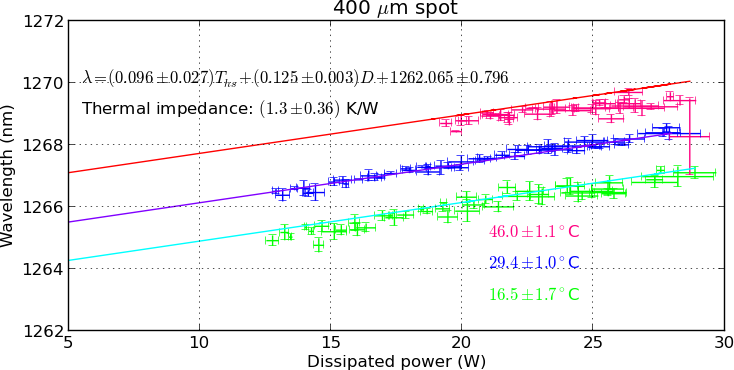
\includegraphics[width=14.5cm]{img/Rth_lambda_spot400um.png}}
\caption{Estimating $\Rth$ with
the method described in section~\ref{sec:rth:lambda}
for three pump spot sizes.
The straight lines correspond
to the fit (\ref{eq:rth_fit}),
taking into account
only the part of linear light-light conversion --
i.e. without the threshold
or roll over segments.}
\label{img:Rth_lambda_spot_scaling}
\end{figure}



\begin{figure}
\centering
\subfigure{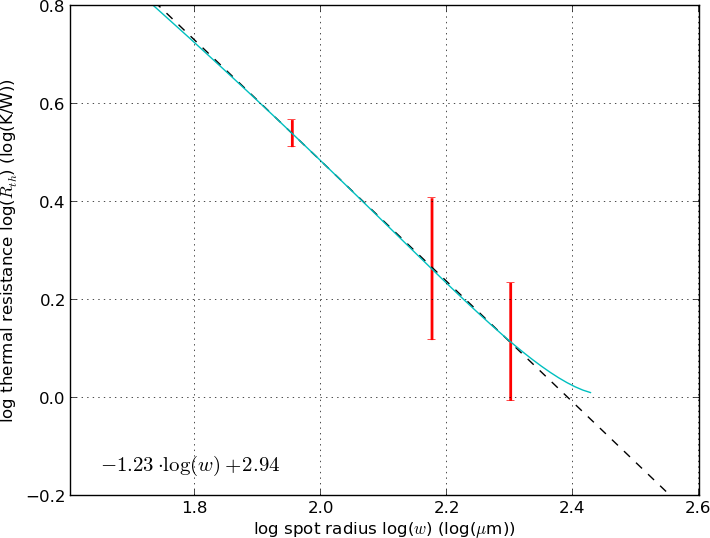
\includegraphics[width=7cm]{img/Rth_spotsizescaling_log.png}}
\subfigure{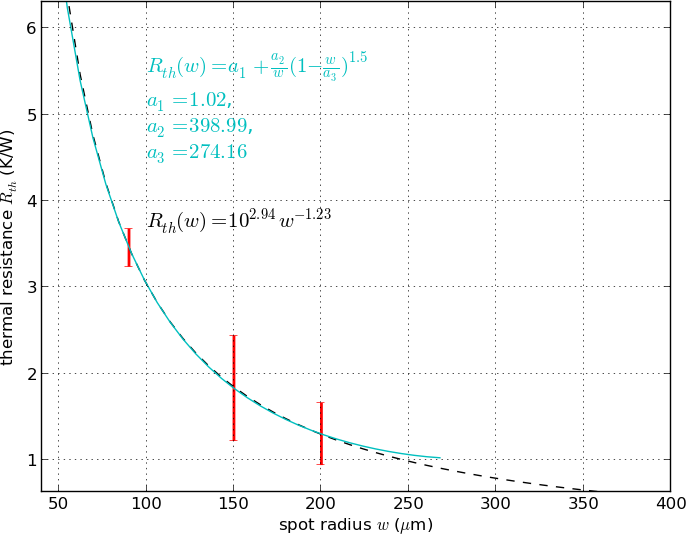
\includegraphics[width=7cm]{img/Rth_spotsizescaling_lin.png}}
\caption{Scaling of thermal resistance
(from Fig.~\ref{img:Rth_lambda_spot_scaling})
with spot size.
Its dependency on spot diameter is expected to be closer to
$(2w)^{-1}$ than $(2w)^{-2}$;
i.e. not to scale with area \cite{Giet2008}.
This is visualized by the slope in the log-log plot (left).
The continuous curve in turquoise shows a fit to
an empirical curve (\ref{eq:Rth_empirical}) \cite{Giet2008,Nakwaski1992}.
Right,
what the fits look like with linear axes.}
\label{img:Rth_spotsizescaling}
\end{figure}

